\chapter{Analiza grafu wynikowego}

\section{Liczba wierzchołków i łuków}

Wynikowy graf ma 3011 wierzchołków i 309748 krawędzi.

\section{Analiza składowych spójności grafu}

Aby zrozumieć strukturę badanego grafu WWW, przeprowadzono analizę składowych spójności. W grafach skierowanych wyróżniamy kilka typów składowych:

\begin{description}
    \item[WCC (Weakly Connected Component)] składowa spójności słaba — zbiór wierzchołków, pomiędzy którymi istnieje ścieżka, jeśli zignorujemy kierunki krawędzi.
    
    \item[SCC (Strongly Connected Component)] składowa spójności silna — zbiór wierzchołków, w którym dla każdej pary $(u,v)$ istnieją ścieżki $u \rightarrow v$ oraz $v \rightarrow u$ z zachowaniem kierunku.
    
    \item[IN] zbiór wierzchołków, z których można dotrzeć do SCC, ale nie można z SCC wrócić do nich.
    
    \item[OUT] zbiór wierzchołków, które można osiągnąć z SCC, ale nie można z nich wrócić do SCC.
    
    \item[TENDRILS / ISLANDS] wierzchołki, które nie należą do SCC, IN ani OUT — np. lokalne połączenia boczne lub całkowicie odizolowane wyspy.
    
    \item[Graf kondensacji SCC ($G_{SCC}$)] graf, w którym każda silnie spójna składowa zostaje zredukowana do jednego wierzchołka. Jest to graf skierowany acykliczny (DAG), reprezentujący zależności pomiędzy składowymi.
\end{description}

\begin{itemize}
    \item \textbf{Liczba słabych składowych spójności (WCC)} wynosi 1, co oznacza, że cały graf jest słabo spójny — można przejść między dowolnymi dwoma wierzchołkami ignorując kierunek krawędzi.

    \item \textbf{Liczba silnych składowych spójności (SCC)} to 1677. Największa z nich (tzw. \textbf{CORE}) zawiera 1251 wierzchołków. CORE odpowiada centralnej części sieci WWW, w której strony są silnie ze sobą połączone w obu kierunkach.

    \item \textbf{IN} zawiera 1750 wierzchołków prowadzących do SCC, ale niedostępnych z niej.

    \item \textbf{OUT} zawiera 7 wierzchołków, do których można dotrzeć z SCC, ale które nie prowadzą z powrotem do niej.

    \item \textbf{TENDRILS / ISLANDS} to tylko 3 wierzchołki — minimalna liczba wskazująca na wysoką spójność globalną.

    \item \textbf{Graf kondensacji} ($G_{SCC}$) zawiera 1677 wierzchołków (po jednej dla każdej SCC) oraz 8280 krawędzi, co świadczy o gęstym połączeniu między komponentami.
\end{itemize}

\begin{figure}[H]
    \centering
    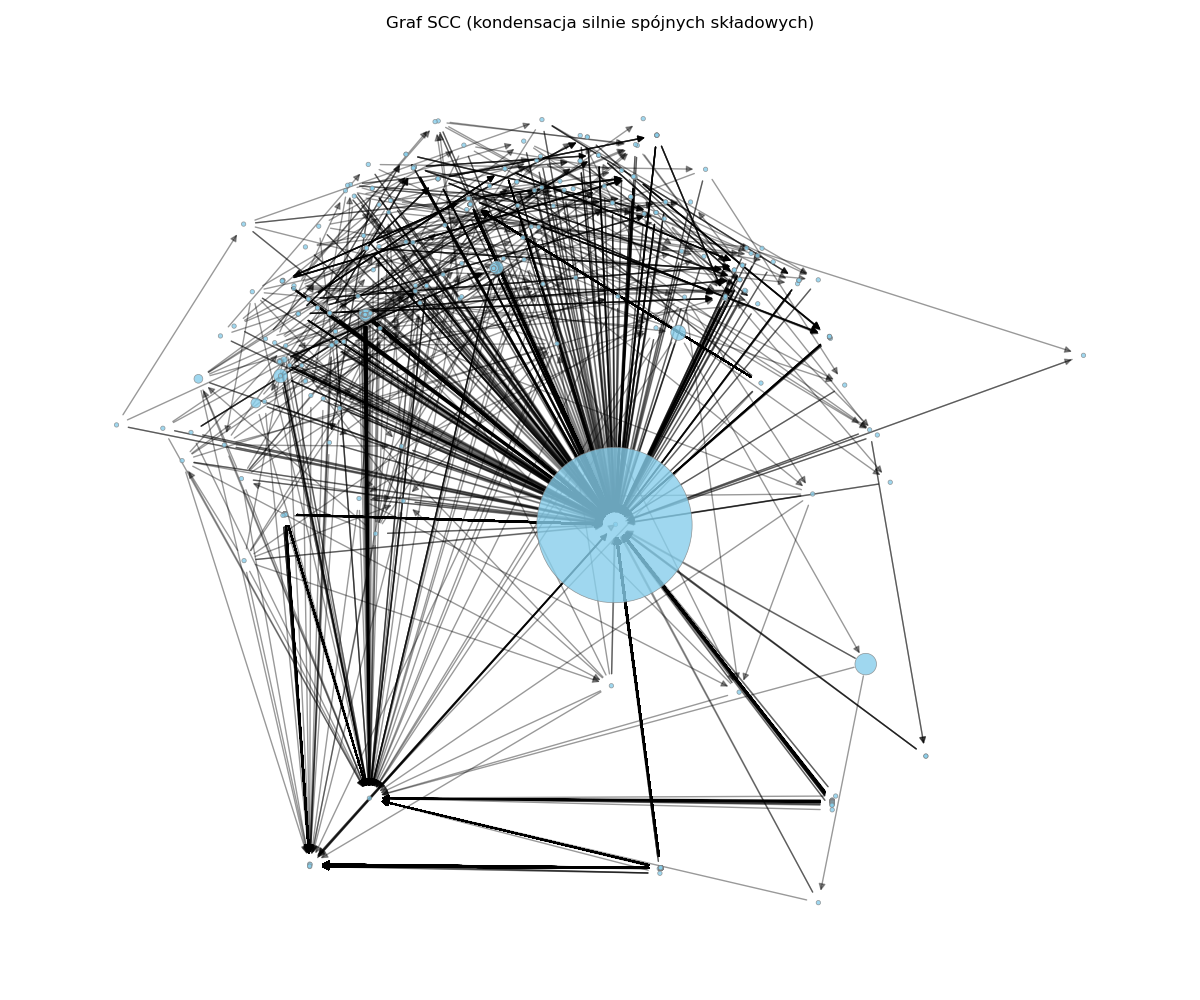
\includegraphics[width=\textwidth]{assets/img_5.png}
    \caption{Graf kondensacji $G_{SCC}$ — każda kropka to jedna silnie spójna składowa}
    \label{fig:g_scc}
\end{figure}

\subsection{Wnioski}

Na podstawie powyższej analizy można zauważyć, że struktura badanego grafu WWW jest zgodna z klasycznym modelem sieci WWW:
\begin{itemize}
    \item Występuje dominująca składowa silnie spójna (CORE), do której prowadzi bardzo duża liczba wierzchołków (IN).
    \item Komponent OUT jest marginalny, co wskazuje na małą liczbę „wyjść” ze strony do innych części sieci.
    \item Niewielka liczba tendrili oraz wysp (ISLANDS) wskazuje na dobrze połączoną strukturę sieci.
    \item Analiza grafu kondensacji pokazuje złożone relacje pomiędzy poszczególnymi silnie spójnymi komponentami.
\end{itemize}

Taka struktura jest charakterystyczna dla rzeczywistych sieci hipertekstowych i potwierdza hipotezę tzw. modelu \textbf{bow-tie}, w którym występują wyraźne obszary CORE, IN i OUT. Model ten jest przydatny do analizy skalowalnych sieci (np. WWW, sieci społecznościowe), ponieważ ujawnia kluczowe komponenty odpowiedzialne za przepływ informacji oraz identyfikuje potencjalne punkty podatne na awarie.

\section{Analiza rozkładów stopni (in-degree, out-degree)}

W celu określenia struktury połączeń w grafie WWW przeanalizowano rozkład stopni wierzchołków — zarówno wejściowych (in-degree), jak i wyjściowych (out-degree). W typowych sieciach skali bezwzględnej oczekuje się, że rozkłady te będą podlegać rozkładowi potęgowemu, czyli:

\[
P(k) \sim k^{-\alpha}
\]

Aby to zweryfikować, wykonano regresję liniową w skali log-log, co pozwala oszacować wykładnik potęgowy $\alpha$ oraz współczynnik dopasowania $R^2$.

\subsection{Rozkład in-degree}

\begin{itemize}
    \item Współczynnik potęgowy: $\alpha \approx 0.43$
    \item Współczynnik determinacji: $R^2 = 0.361$
\end{itemize}

\begin{figure}[H]
    \centering
    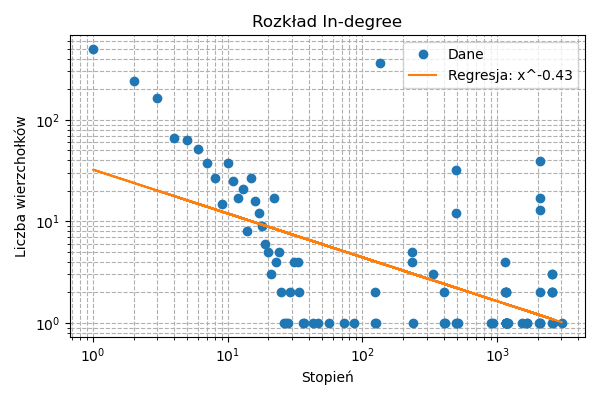
\includegraphics[width=\textwidth]{assets/img_6.png}
    \caption{Rozkład in-degree w skali log-log z dopasowaną funkcją potęgową}
\end{figure}

Pomimo pewnej tendencji do zachowania rozkładu potęgowego, niskie $R^2$ wskazuje, że dopasowanie nie jest idealne. Może to świadczyć o obecności zakłóceń (np. odcięcia w zakresie małych lub bardzo dużych stopni), lub że sieć nie jest klasycznie skali bezwzględna.

\subsection{Rozkład out-degree}

\begin{itemize}
    \item Współczynnik potęgowy: $\alpha \approx -0.34$ (odwrotność, ponieważ rośnie)
    \item Współczynnik determinacji: $R^2 = 0.069$
\end{itemize}

\begin{figure}[H]
    \centering
    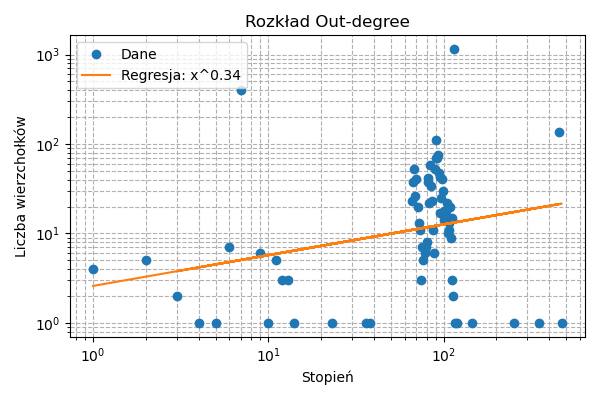
\includegraphics[width=\textwidth]{assets/img_7.png}
    \caption{Rozkład out-degree w skali log-log z dopasowaną funkcją potęgową}
\end{figure}

Dla rozkładu out-degree uzyskano bardzo niskie $R^2$, co oznacza słabe dopasowanie modelu potęgowego do danych. Może to wskazywać, że stopnie wyjściowe są bardziej jednorodne (np. wiele stron ma podobną liczbę linków wychodzących), co zaburza rozkład potęgowy.

\subsection{Wnioski}

Rozkłady stopni w badanym grafie tylko częściowo spełniają cechy sieci skali bezwzględnej. Chociaż rozkład in-degree wykazuje lekką tendencję do zachowania funkcji potęgowej, to out-degree jest znacznie mniej uporządkowany. Możliwe przyczyny to:
\begin{itemize}
    \item specyfika lokalnej struktury strony uczelni (dużo stron głównych linkujących do wielu zasobów),
    \item ograniczenia crawl (limit liczby stron),
    \item zaburzenia wynikające z dynamicznych linków lub zasobów zewnętrznych.
\end{itemize}

\section{Analiza najkrótszych ścieżek w grafie}

Aby zbadać strukturę odległości w sieci, przeanalizowano najkrótsze ścieżki pomiędzy wszystkimi parami wierzchołków w największej silnie spójnej składowej (SCC). W tego typu grafach często występuje efekt tzw. \textit{małego świata}, czyli niska średnia odległość pomiędzy wierzchołkami.

\subsection{Wyniki dla największej SCC}

\begin{itemize}
    \item Średnia odległość pomiędzy parami wierzchołków: $\mathbf{2{,}67}$
    \item Średnica grafu (najdłuższa najkrótsza ścieżka): $\mathbf{7}$
\end{itemize}

\subsection{Rozkład średnich odległości}

Dla każdego wierzchołka obliczono średnią odległość do pozostałych. Histogram tych wartości przedstawiono na rysunku~\ref{fig:avg_dist_hist}. Następnie przeprowadzono dopasowanie funkcji potęgowej w skali log-log:

\[
f(x) \sim x^{-9{,}23}, \quad R^2 = 0{,}76
\]

Uzyskane dopasowanie wskazuje na stosunkowo dobre odwzorowanie rozkładu funkcją potęgową, co sugeruje obecność centralnych węzłów o krótkich ścieżkach do reszty grafu.

\begin{figure}[H]
    \centering
    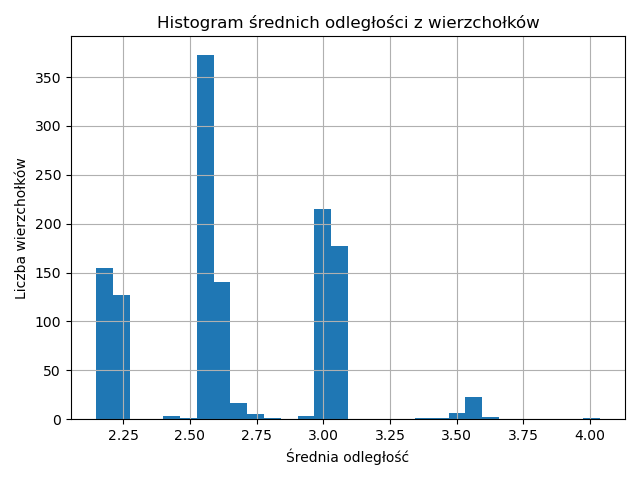
\includegraphics[width=\textwidth]{assets/img_8.png}
    \caption{Histogram średnich odległości z wierzchołków}
    \label{fig:avg_dist_hist}
\end{figure}

\subsection{Rozkład promieni}

Promień wierzchołka to największa odległość do innego wierzchołka w jego komponentach. Histogram promieni przedstawia rysunek~\ref{fig:radius_hist}.

\begin{figure}[H]
    \centering
    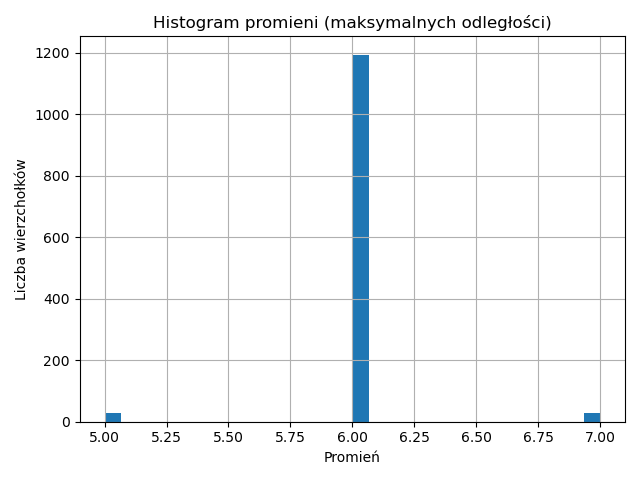
\includegraphics[width=\textwidth]{assets/img_9.png}
    \caption{Histogram promieni (maksymalnych odległości)}
    \label{fig:radius_hist}
\end{figure}

Zdecydowana większość wierzchołków ma promień równy 6, co sugeruje dobrą spójność i relatywnie płaską strukturę wewnątrz głównego komponentu SCC.

\subsection{Wnioski}

Analiza odległości potwierdza obecność zjawiska \textbf{małego świata} w strukturze grafu — większość stron jest osiągalna w maksymalnie kilku krokach. Histogramy wskazują na spójność i przewidywalność rozkładu odległości. Wyniki te są charakterystyczne dla naturalnie powstających grafów WWW.

\section{Analiza współczynników klasteryzacji}

Współczynniki klasteryzacji opisują, w jakim stopniu sąsiedzi danego wierzchołka również są ze sobą połączeni, czyli jak lokalnie „gęsta” jest struktura grafu. Dla grafu WWW można je traktować jako miarę grupowania stron o podobnej tematyce lub powiązanych funkcjonalnie.

Wyróżniamy dwa typy klasteryzacji:
\begin{itemize}
    \item \textbf{Lokalny współczynnik klasteryzacji ($C_v$)} — liczony osobno dla każdego wierzchołka jako stosunek liczby istniejących połączeń między sąsiadami do liczby możliwych połączeń.
    \item \textbf{Globalny współczynnik klasteryzacji ($C$)} — średnia z lokalnych współczynników lub liczony jako stosunek trzykątów do trójek możliwych.
\end{itemize}

\subsection{Wyniki}

\begin{itemize}
    \item Globalny współczynnik klasteryzacji: $\mathbf{0{,}6949}$
    \item Liczba wierzchołków z $C_v > 0$: $\mathbf{3008}$
\end{itemize}

Histogram lokalnych współczynników klasteryzacji przedstawiono na rysunku~\ref{fig:clust_hist}. Dane te sugerują, że znaczna część wierzchołków ma wysoki poziom lokalnego grupowania, co wskazuje na obecność silnie powiązanych podstruktur w grafie.

\begin{figure}[H]
    \centering
    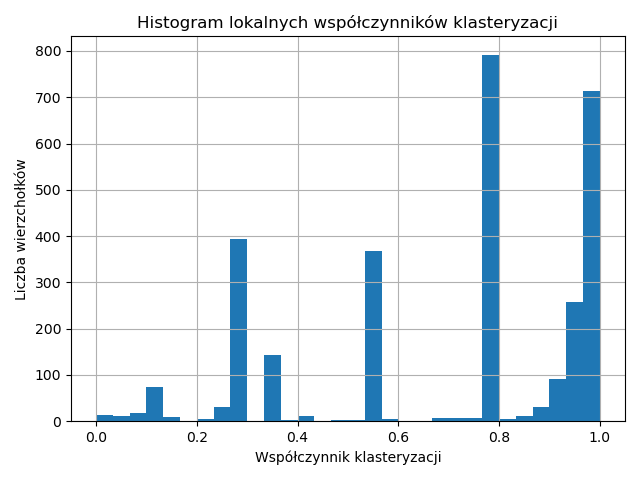
\includegraphics[width=\textwidth]{assets/img_10.png}
    \caption{Histogram lokalnych współczynników klasteryzacji}
    \label{fig:clust_hist}
\end{figure}

\subsection{Rozkład klasteryzacji w skali log-log}

Aby ocenić, czy wartości lokalnego współczynnika klasteryzacji podlegają rozkładowi potęgowemu, przeprowadzono analizę regresji w skali log-log. Otrzymano następujące wyniki:

\[
f(x) \sim x^{0{,}37}, \quad R^2 = 0{,}03
\]

Niski współczynnik determinacji $R^2$ świadczy o bardzo słabym dopasowaniu modelu potęgowego. Oznacza to, że rozkład lokalnych współczynników klasteryzacji nie podlega funkcji potęgowej.

\begin{figure}[H]
    \centering
    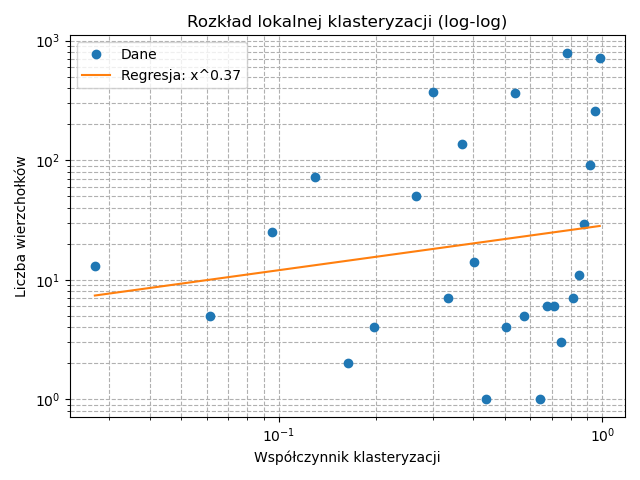
\includegraphics[width=\textwidth]{assets/img_11.png}
    \caption{Rozkład lokalnej klasteryzacji (log-log) z regresją potęgową}
    \label{fig:clust_loglog}
\end{figure}

\subsection{Wnioski}

Analiza współczynników klasteryzacji wykazuje, że:
\begin{itemize}
    \item Graf cechuje się wysokim globalnym poziomem klasteryzacji ($C \approx 0{,}69$), co jest typowe dla grafów sieciowych (np. WWW, sieci społecznościowe).
    \item Większość wierzchołków posiada dodatni współczynnik lokalny, często bliski 1 — co wskazuje na obecność licznych lokalnych struktur typu „kliki”.
    \item Rozkład lokalnej klasteryzacji nie podlega prawu potęgowemu, co może być skutkiem ograniczeń topologicznych strony uczelni (np. sztywne szablony, sekcje z wieloma wewnętrznymi linkami).
\end{itemize}

\section{Analiza spójności wierzchołkowej}

Spójność wierzchołkowa określa minimalną liczbę wierzchołków, które należy usunąć z grafu, aby stał się niespójny (czyli został rozdzielony na co najmniej dwie osobne składowe).

\begin{itemize}
    \item Jeżeli spójność wierzchołkowa wynosi $k = 1$, to istnieje co najmniej jeden \textbf{punkt artykulacji} — wierzchołek, którego usunięcie prowadzi do rozspojenia grafu.
    \item Jeżeli $k = 2$, to potrzebne są co najmniej dwa usunięcia (tzw. \textbf{pary wierzchołków rozspajających}).
\end{itemize}

W analizowanym grafie największej silnie spójnej składowej (SCC) uzyskano następujące wyniki:

\begin{itemize}
    \item \textbf{Spójność wierzchołkowa:} $1$
    \item Znaleziono $2$ \textbf{punkty artykulacji}, których usunięcie rozdziela graf:
    \begin{itemize}
        \item \url{https://www.um.edu.mt/research/ethics/researchethicsatum/}
        \item \url{https://www.um.edu.mt/}
    \end{itemize}
\end{itemize}

\subsection{Interpretacja}

Obecność zaledwie dwóch punktów artykulacji oznacza, że graf jest ogólnie dobrze połączony, ale zawiera krytyczne wierzchołki, których usunięcie skutkuje przerwaniem ciągłości sieci. Są to zazwyczaj centralne lub nadrzędne strony (np. strona główna uczelni), do których prowadzi wiele połączeń i które pośredniczą w dostępie do innych podstron.

\subsection{Wnioski}

\begin{itemize}
    \item Spójność wierzchołkowa na poziomie $k = 1$ świadczy o względnej odporności strukturalnej, choć nie całkowitej — atak na jeden kluczowy wierzchołek może zakłócić komunikację w obrębie grafu.
    \item Zidentyfikowane punkty artykulacji mogą stanowić potencjalne punkty awarii lub „wąskie gardła” w strukturze sieci.
    \item W kontekście projektowania struktur WWW warto dążyć do większej nadmiarowości połączeń, aby zminimalizować wpływ usunięcia jednego centralnego zasobu.
\end{itemize}

